\documentclass[11pt,a4paper]{article}
\usepackage[utf8]{inputenc}
\usepackage[T1]{fontenc}
\usepackage{mathptmx}
\usepackage[a4paper,top=1.8cm,bottom=1.8cm,left=2cm,right=2cm]{geometry}
\usepackage{microtype}
\usepackage{titlesec}
\usepackage{enumitem}
\usepackage[font=small,labelfont=bf,labelsep=period]{caption}
\usepackage{booktabs}
\usepackage{tabularx}
\usepackage{fancyhdr}
\usepackage{xcolor}
\usepackage{tikz}
\usetikzlibrary{positioning,arrows.meta}

\renewcommand{\tablename}{Tabla}
\renewcommand{\figurename}{Figura}
\renewcommand{\refname}{Referencias}
\newcommand{\sq}[1]{\texttt{#1}}
\newcommand{\cod}[1]{\texttt{\small #1}}

\titleformat{\section}{\large\bfseries}{\thesection.}{0.5em}{}
\titlespacing*{\section}{0pt}{7pt}{3pt}
\titleformat{\subsection}{\normalsize\bfseries\itshape}{}{0em}{}
\titlespacing*{\subsection}{0pt}{4pt}{1pt}
\setlist{itemsep=0.5pt,topsep=1.5pt,parsep=0pt,leftmargin=1.2em}
\setlength{\parskip}{2.5pt}
\setlength{\parindent}{0pt}

\pagestyle{fancy}
\fancyhf{}
\lhead{\small Bioinformática -- Del ADN a la proteína}
\rhead{\small Grupo 19 -- ULPGC, curso 2026/2027}
\cfoot{\small\thepage}
\renewcommand{\headrulewidth}{0.4pt}

\begin{document}

\begin{center}
{\Large\bfseries Del ADN a la proteína: replicación, transcripción,\\[1pt] traducción y splicing con Biopython}\\[5pt]
{\small Universidad de Las Palmas de Gran Canaria · Grado en Ciencia e Ingeniería de Datos}\\[1pt]
{\small Bioinformática · Profesora: María Dolores Afonso Suárez · Curso 2026/2027}\\[1pt]
{\small Grupo 19: \textbf{Hugo Amador Hidalgo y Sara Lillo} · Repositorio: \sq{github.com/hugoamadoor/BIOINFORMATICA}}
\end{center}
\vspace{-6pt}

\section*{Código y reproducibilidad}
Cada ejercicio tiene un script en \sq{src/} que resuelve el caso del enunciado y lo compara con el resultado obtenido a mano. Las funciones comunes (complementaria, replicación, transcripción, búsqueda de la ORF y traducción) están en \sq{src/dogma.py} y usan \sq{Bio.Seq} y \sq{Bio.SeqIO} \cite{biopython}. Los resultados manuales están además fijados como pruebas en \sq{tests/test\_dogma.py} (6 pruebas, \sq{pytest}). El README del repositorio explica la instalación y el uso.

\section{Replicación del ADN}
\textbf{Hebras nuevas.} La replicación es semiconservativa \cite{ws,ms}: se separan las dos hebras y cada una sirve de molde para sintetizar su complementaria en sentido 5$'\!\to$3$'$. Se obtienen dos moléculas hijas idénticas a la parental, cada una con una hebra antigua y una nueva:
\begin{center}\small
\begin{tabular}{lll}
\toprule
 & Hebra parental (molde) & Hebra nueva \\
\midrule
Hija 1 & 5$'$-\sq{ATG CCG TTA GCT}-3$'$ & 3$'$-\sq{TAC GGC AAT CGA}-5$'$ \quad(= 5$'$-\sq{AGCTAACGGCAT}-3$'$)\\
Hija 2 & 3$'$-\sq{TAC GGC AAT CGA}-5$'$ & 5$'$-\sq{ATG CCG TTA GCT}-3$'$\\
\bottomrule
\end{tabular}
\end{center}
Si la horquilla avanza de izquierda a derecha, la hebra nueva que se forma sobre el molde inferior crece hacia la horquilla. Es la \emph{conductora} y se sintetiza de forma continua. La que se forma sobre el molde superior crece en sentido contrario. Es la \emph{retardada} y se sintetiza en fragmentos de Okazaki.

\textbf{Función de las enzimas.}
\begin{itemize}
\item \textbf{Helicasa:} rompe los puentes de hidrógeno entre las bases y abre la horquilla gastando ATP. Las proteínas SSB mantienen separadas las hebras sencillas, y la topoisomerasa alivia el superenrollamiento que se acumula por delante.
\item \textbf{Primasa:} es una ARN polimerasa que sintetiza un cebador corto de ARN, necesario porque la ADN polimerasa no puede empezar una cadena desde cero. Hace falta un cebador en la hebra conductora y uno por cada fragmento de Okazaki.
\item \textbf{ADN polimerasa:} añade desoxinucleótidos al extremo 3$'$-OH siguiendo la complementariedad A--T/G--C, siempre en sentido 5$'\!\to$3$'$. Su actividad exonucleasa 3$'\!\to$5$'$ corrige errores. En \textit{E.\,coli}, la Pol III sintetiza y la Pol I sustituye los cebadores por ADN.
\item \textbf{Ligasa:} sella las mellas entre fragmentos de Okazaki formando el último enlace fosfodiéster.
\end{itemize}

\textbf{Reflexión: error no corregido.} La polimerasa por sí sola se equivoca aproximadamente una vez cada $10^4$--$10^5$ nucleótidos. La corrección de pruebas y la reparación de desapareamientos (MMR) bajan esa tasa a unos $10^{-9}$--$10^{-10}$ por nucleótido y ronda. Si un error escapa a ambos mecanismos, en la ronda siguiente la hebra errónea sirve de molde y el cambio queda fijado con su pareja correcta: 1 de las 4 moléculas lleva ya una \emph{mutación} estable y heredable. Su efecto depende del codón afectado. Puede ser silenciosa (\sq{GCT}$\to$\sq{GCC}, Ala), de cambio de sentido (\sq{TTA}$\to$\sq{TCA}, Leu$\to$Ser) o sin sentido. \sq{ej1\_replicacion.py} simula este último caso: \sq{TTA}$\to$\sq{TAA} convierte el péptido \sq{MPLA} en \sq{MP}. Una inserción o deleción desplazaría además la pauta de lectura.

\textbf{Código.} \sq{ej1\_replicacion.py} genera la complementaria con \sq{Seq.reverse\_complement()} y confirma que las dos hebras nuevas coinciden con las obtenidas a mano.

\section{Transcripción del ADN a ARN}
\textbf{Cadena molde.} La ARN polimerasa lee el molde en sentido 3$'\!\to$5$'$ y sintetiza el ARN en sentido 5$'\!\to$3$'$. Para que el transcrito empiece por el codón de inicio AUG, el molde debe ser la hebra inferior, 3$'$-\sq{TAC GGA CTT ACG}-5$'$. La superior es la hebra \emph{codificante}: tiene la misma secuencia que el ARN, con T en lugar de U.

\textbf{Transcrito:} 5$'$-\sq{AUG CCU GAA UGC}-3$'$, que se traduciría como Met--Pro--Glu--Cys. No tiene codón de paro, así que es un fragmento.

\textbf{Promotor y región codificante.} Los 12 nucleótidos del enunciado son \emph{región codificante}: empiezan en el ATG, que marca el inicio de la \emph{traducción}. El \emph{promotor} no aparece en la secuencia. Estaría aguas arriba (en el lado 5$'$ de la hebra codificante), antes del sitio de inicio de la transcripción (+1). En bacterias está formado por las cajas $-10$ (\sq{TATAAT}) y $-35$ (\sq{TTGACA}); en eucariotas, por la caja TATA (hacia $-25/-30$) y otros elementos que reconoce la ARN polimerasa II. Entre el +1 y el ATG quedaría la 5$'$UTR.

\textbf{Experimento de orientación} (\sq{ej2\_transcripcion.py}, que lee un FASTA). \sq{Seq.transcribe()} solo cambia T por U, es decir, supone que se le da la hebra codificante. Si se le pasa otra cosa, el resultado es incorrecto:
\begin{center}\small
\begin{tabular}{lll}
\toprule
Entrada & ARN obtenido & Traducción \\
\midrule
Codificante 5$'\!\to$3$'$ (correcto) & \sq{AUGCCUGAAUGC} & \sq{MPEC}\\
Molde 5$'\!\to$3$'$ sin invertir ni complementar & \sq{GCAUUCAGGCAU} & \sq{AFRH}\\
Complemento sin invertir (molde leído 3$'\!\to$5$'$) & \sq{UACGGACUUACG} & \sq{YGLT}\\
\bottomrule
\end{tabular}
\end{center}
Por eso, con la hebra molde hay que hacer \sq{reverse\_complement()} antes de transcribir. El script lo hace con la opción \sq{--hebra molde}.

\section{Traducción del ARNm a proteína}
En 5$'$-\sq{AUG UAU GCU UAA}-3$'$, el codón de inicio es \sq{AUG} (Met) y el de paro es \sq{UAA} (ocre). El resultado es el tripéptido \textbf{Met--Tyr--Ala} (\sq{MYA}). \sq{Bio.Seq.translate()} devuelve \sq{MYA*} y, con \sq{to\_stop=True}, \sq{MYA}, igual que a mano.

\textbf{AUG$\to$GUG.} En eucariotas, el ribosoma que recorre el ARNm pasaría de largo por el GUG y empezaría en el siguiente AUG. Aquí ese AUG está en la posición 5, fuera de fase (\sq{GUG U\underline{AUG} CUU AA}), así que se leería otra pauta (Met--Leu\dots) y no se obtendría el péptido original. Biopython lo refleja: con la tabla estándar y \sq{cds=True} rechaza \sq{GUG} como inicio. En bacterias, en cambio, GUG es un codón de inicio alternativo que usa una minoría de genes. El ARNt iniciador sigue colocando (f)Met, de modo que con la tabla 11 se obtiene \sq{MYA}, aunque con menor eficiencia de inicio.

\textbf{Pérdida del codón de paro} (p.\,ej. \sq{UAA}$\to$\sq{CAA}, Gln). El ribosoma sigue leyendo la 3$'$UTR hasta el siguiente paro en fase y produce una proteína con el extremo C alargado. Con una 3$'$UTR hipotética, el script obtiene \sq{MYAQAG}. Si no aparece ningún paro antes de la cola poli(A), el ARNm se degrada por la vía \emph{non-stop decay}. La proteína alargada puede plegarse mal o ser degradada.

\section{Splicing alternativo}
Se consideran un gen de 5 exones con los exones 1 y 5 constitutivos y tres combinaciones alternativas además de la completa. Para probarlas, \sq{ej4\_splicing.py} usa un gen de juguete con exones de 24, 20, 22, 21 y 24\,nt:
\begin{center}\small
\begin{tabularx}{\linewidth}{llX}
\toprule
Isoforma & Pauta de lectura & Proteína resultante \\
\midrule
1-2-3-4-5 & correcta & completa, 36 aa (referencia)\\
1-2-3-5 & correcta (21 nt $\equiv 0$) & 29 aa: le faltan los 7 aa del exón 4 y el resto no cambia \\
1-2-4-5 & desplazada (se salta 22 nt) & 27 aa: extremo C distinto y paro prematuro en el último exón \\
1-3-5 & desplazada (se saltan 41 nt) & 15 aa: truncada; el paro cae junto a la última unión \\
\bottomrule
\end{tabularx}
\end{center}
\textbf{Diferencias esperables.} Si el fragmento saltado es múltiplo de 3, se obtiene una proteína más corta a la que le falta un segmento, por ejemplo un dominio de unión, una señal de localización o un dominio transmembrana (que daría una forma soluble). Si no lo es, la pauta se desplaza, cambia todo lo que queda aguas abajo y suele aparecer un paro prematuro. Si ese paro queda a más de 50--55\,nt de la última unión exón--exón, el ARNm se degrada por NMD. Si no, se produce una proteína truncada. En el gen de juguete, los paros quedan cerca de la última unión y ninguna isoforma activaría el NMD.

\textbf{¿Por qué aumenta la diversidad sin más genes?} Con 3 exones opcionales hay ya $2^3=8$ isoformas posibles. A eso se suman los exones mutuamente excluyentes, los sitios 5$'$/3$'$ alternativos y la retención de intrones. En humanos hay unos 20\,000 genes codificantes, y más del 90\,\% de los que tienen varios exones presentan splicing alternativo \cite{wang,pan}. Cada tejido y cada etapa del desarrollo elige isoformas mediante reguladores como las proteínas SR y las hnRNP, de modo que un mismo gen da proteínas con funciones distintas.

\textbf{FGFR2 en Ensembl} \cite{ensembl}. El gen (ENSG00000066468, cromosoma 10, hebra $-$) tiene 59 transcritos, de los que 38 codifican proteína, con 31 longitudes distintas (de 56 a 822\,aa). El canónico (MANE Select) es FGFR2-206 (ENST00000358487), con 18 exones y 821\,aa. Uno de los más largos, FGFR2-215, tiene 822\,aa. Sus isoformas más estudiadas se diferencian en dos exones mutuamente excluyentes que codifican la mitad del tercer dominio Ig: \textbf{IIIb}, epitelial, que une FGF7 y FGF10, y \textbf{IIIc}, mesenquimal, que une FGF2 entre otros. Un solo cambio de exón altera qué ligandos reconoce el receptor y, por tanto, su papel en el desarrollo. Las mutaciones en esta región se asocian a craneosinostosis (síndromes de Crouzon y Apert). La tabla completa de transcritos se obtiene con \sq{ej4\_splicing.py --ensembl FGFR2}.

\section{Introducción a las proteínas}
En Met--Ile--Ser--Gly--Val--Lys--His, el \textbf{extremo N} es la \textbf{Met} (grupo $\alpha$-amino libre) y el \textbf{extremo C} es la \textbf{His} (grupo $\alpha$-carboxilo libre). Por convenio, los péptidos se escriben de N a C, que es el orden en que los sintetiza el ribosoma. \sq{ej5\_proteinas.py} clasifica los restos con la escala de Kyte--Doolittle: Met, Ile y Val son hidrofóbicos, Ser es polar, Gly es especial y Lys e His son básicos. El péptido tiene GRAVY $=+0{,}33$ y pI $\approx 8{,}5$.

\textbf{Orden y estructura.} La secuencia contiene la información necesaria para el plegamiento \cite{anfinsen}. El efecto hidrofóbico entierra los restos apolares en el núcleo y deja los polares expuestos. Además, el patrón de restos favorece unas estructuras u otras: Ala, Leu, Glu o Met tienden a formar hélices $\alpha$; Val, Ile o Tyr, hebras $\beta$; y Gly y Pro las interrumpen. Con los mismos aminoácidos en otro orden, la proteína se pliega de otra manera.

\textbf{Mutación hidrofóbico$\to$hidrofílico en el núcleo.} Enterrar una carga o un grupo polar sin pareja cuesta energía y rompe el empaquetamiento de van der Waals. La proteína se desestabiliza y puede plegarse mal, agregarse, ser degradada por el proteasoma o perder su función. En el script, la mutación I2K hace que el GRAVY pase de $+0{,}33$ a $-0{,}87$.

\textbf{PDB} \cite{pdb}. En la desoxihemoglobina humana (\sq{4HHB}), cada subunidad adopta el plegamiento globina de 8 hélices $\alpha$ (A--H) y no tiene láminas $\beta$. En cambio, la GFP (\sq{1EMA}) es un barril de 11 hebras $\beta$. Una sola mutación puntual en la cadena $\beta$ de la hemoglobina, Glu6Val, crea en la superficie una zona hidrofóbica que hace polimerizar la desoxi-HbS (anemia falciforme). Es el caso inverso al del núcleo, pero muestra el mismo principio. \sq{ej5\_proteinas.py --pdb} resume las hélices y hebras de cualquier fichero descargado del PDB.

\section{Actividad integradora: del ADN a la proteína}
Se ha usado la \textbf{CDS de la insulina humana} (\textit{INS}, transcrito ENST00000381330.5 de Ensembl, GRCh38): 333\,nt, 64,6\,\% de GC, \sq{ATG}\dots\sq{TAG} y 111 codones. \sq{ej6\_pipeline.py} encadena los tres procesos y va informando de cada paso por pantalla y en \sq{resultados/pipeline.log}:

\begin{center}
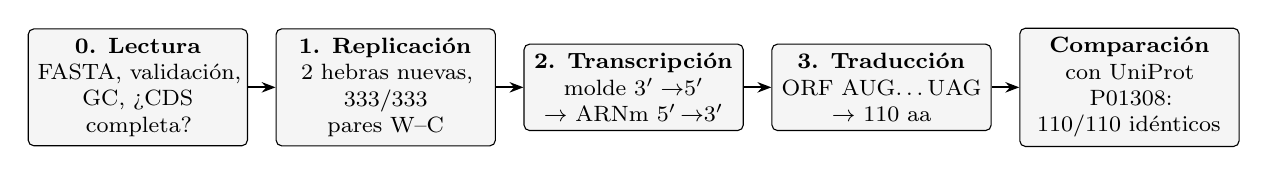
\begin{tikzpicture}[node distance=0.35cm, font=\footnotesize,
  caja/.style={draw, rounded corners=2pt, align=center, minimum height=0.95cm, text width=2.55cm, fill=gray!8},
  flecha/.style={-{Stealth[length=5pt]}, thick}]
\node[caja] (a) {\textbf{0. Lectura}\\FASTA, validación,\\GC, ¿CDS completa?};
\node[caja, right=of a] (b) {\textbf{1. Replicación}\\2 hebras nuevas,\\333/333 pares W--C};
\node[caja, right=of b] (c) {\textbf{2. Transcripción}\\molde 3$'\!\to$5$'$\\$\to$ ARNm 5$'\!\to$3$'$};
\node[caja, right=of c] (d) {\textbf{3. Traducción}\\ORF AUG\dots UAG\\$\to$ 110 aa};
\node[caja, right=of d] (e) {\textbf{Comparación}\\con UniProt P01308:\\110/110 idénticos};
\draw[flecha] (a)--(b); \draw[flecha] (b)--(c); \draw[flecha] (c)--(d); \draw[flecha] (d)--(e);
\end{tikzpicture}
\end{center}

\textbf{Resultados.} (1) Las dos hebras nuevas son 5$'$-\sq{CTAGTTGCAG\dots GGGCCAT}-3$'$, sintetizada sobre el molde codificante, y 5$'$-\sq{ATGGCCCTGT\dots CAACTAG}-3$'$, sintetizada sobre el molde. Las dos moléculas hijas son idénticas a la parental. (2) El ARNm es 5$'$-\sq{AUGGCCCUGUGG\dots UGCAACUAG}-3$'$. (3) La proteína es la \textbf{preproinsulina} (110\,aa, 12,0\,kDa, pI 5,22) y coincide al 100\,\% con UniProt P01308 \cite{uniprot}. El dogma central termina aquí, pero la hormona activa no: tras la traducción se elimina el péptido señal (1--24) y se corta el péptido C (57--87), y las cadenas B (25--54) y A (90--110) quedan unidas por puentes disulfuro. La secuencia del gen no basta para describir la proteína funcional.

\textbf{Reflexión: ¿qué punto es más vulnerable?} Depende de si se mira la frecuencia o las consecuencias. La tasa de error es mayor en la traducción ($\sim10^{-4}$--$10^{-3}$ por codón) y en la transcripción ($\sim10^{-5}$--$10^{-4}$) que en la replicación ($\sim10^{-9}$--$10^{-10}$). Sin embargo, esos errores son transitorios: afectan a una molécula de ARN o de proteína que se sustituye. Un error de \emph{replicación} no corregido, en cambio, se vuelve una mutación permanente, pasa a las células hijas y altera \emph{todas} las copias de ARNm y de proteína que se produzcan a partir de él. Por eso la replicación es el punto más vulnerable en cuanto a efecto sobre la función, y también el que tiene más mecanismos de control. En la insulina, por ejemplo, hay mutaciones del gen \textit{INS} que impiden que la proinsulina se pliegue bien y causan diabetes neonatal.

\small
\begin{thebibliography}{9}\setlength{\itemsep}{0pt}
\bibitem{biopython} Cock, P.\,J.\,A. \textit{et al.} (2009). Biopython. \textit{Bioinformatics} 25, 1422--1423.
\bibitem{ws} Watson, J.\,D. y Crick, F.\,H.\,C. (1953). Genetical implications of the structure of DNA. \textit{Nature} 171, 964--967.
\bibitem{ms} Meselson, M. y Stahl, F.\,W. (1958). The replication of DNA in \textit{E.\,coli}. \textit{PNAS} 44, 671--682.
\bibitem{wang} Wang, E.\,T. \textit{et al.} (2008). Alternative isoform regulation in human tissue transcriptomes. \textit{Nature} 456, 470--476.
\bibitem{pan} Pan, Q. \textit{et al.} (2008). Deep surveying of alternative splicing complexity in the human transcriptome. \textit{Nat. Genet.} 40, 1413--1415.
\bibitem{ensembl} Harrison, P.\,W. \textit{et al.} (2024). Ensembl 2024. \textit{Nucleic Acids Res.} 52, D891--D899.
\bibitem{anfinsen} Anfinsen, C.\,B. (1973). Principles that govern the folding of protein chains. \textit{Science} 181, 223--230.
\bibitem{pdb} Berman, H.\,M. \textit{et al.} (2000). The Protein Data Bank. \textit{Nucleic Acids Res.} 28, 235--242.
\bibitem{uniprot} UniProt Consortium. Entrada P01308 (INS\_HUMAN). \sq{https://www.uniprot.org/uniprotkb/P01308}
\end{thebibliography}

\end{document}
